% This must be in the first 5 lines to tell arXiv to use pdfLaTeX, which is strongly recommended.
\pdfoutput=1
% In particular, the hyperref package requires pdfLaTeX in order to break URLs across lines.

\documentclass[11pt]{article}

% Remove the "review" option to generate the final version.
\usepackage[review]{ACL2023}

% Standard package includes
\usepackage{times}
\usepackage{latexsym}
\usepackage{amsmath}
\usepackage{float}
\usepackage{graphicx}
\usepackage[justification=centering]{caption}

% For proper rendering and hyphenation of words containing Latin characters (including in bib files)
\usepackage[T1]{fontenc}
% For Vietnamese characters
% \usepackage[T5]{fontenc}
% See https://www.latex-project.org/help/documentation/encguide.pdf for other character sets

% This assumes your files are encoded as UTF8
\usepackage[utf8]{inputenc}

% This is not strictly necessary, and may be commented out.
% However, it will improve the layout of the manuscript,
% and will typically save some space.
\usepackage{microtype}

% This is also not strictly necessary, and may be commented out.
% However, it will improve the aesthetics of text in
% the typewriter font.
\usepackage{inconsolata}


% If the title and author information does not fit in the area allocated, uncomment the following
%
%\setlength\titlebox{<dim>}
%
% and set <dim> to something 5cm or larger.

\title{Select-Top-K: \\ Reducing the Memory Use of Naive Bayes}

\author{Adrian Gushin \\
  Emory University / 1526 Harrison Avenue \\
  \texttt{agushin@emory.edu}}

\begin{document}
{\makeatletter\acl@finalcopytrue
  \maketitle
}
\begin{abstract}
Generative Naive Bayes methods are a state of the art natural language processing technique used for performing sentiment analysis. Achieving a high-performance model requires ample training data, which could create memory management concerns if the dataset is sufficiently large. This paper will explore two strategies to reduce the number of words in each training sample and therefore address storage concerns and will compare models trained on these limited datasets to a model trained on the full, unmodified dataset. For the data used in this project, I find that the size of a given training sample can be reduced by a factor of 0.522 while maintaining comparable results to the full dataset.
\end{abstract}

\section{Introduction}

Sentiment analysis is a natural language processing technique in which an automated system predicts the emotional resonance of input text. Sentiment analysis tasks range from simple binary classification of text into positive and negative groups to predicting a text's dominant emotion. Examples of such experiments include those by \citet{go2009twitter} and \citet{saravia2018carer} respectively. 

A ubiquitous and state of the art method for performing sentiment analysis is the Naive Bayes algorithm \citep{khurana2023natural}. Given a set of classes $C = \{c_1, c_2,\dots,c_n\}$ and a set of training documents $D = \{d_1, d_2,\dots,d_m\}$, the algorithm will produce and maintain a conditional probability distribution across each word in $D$ conditioned on each class $C$. Words that appear in one class but not others are typically handled using the add-$\alpha$ smoothing technique \citep{cherian2017heart}. The algorithm performs classification by applying each of the conditional probability distributions to an input text and classifying the text based on which probability is higher.

Because of this reliance on its conditional probability distributions, it is paramount to ensure that the Naive Bayes model has large quantities of quality training data. This step will ensure that the conditional distributions are as accurate as possible and greatly improves the quality of the model \citep{islam2007investigating}. The importance of a large training dataset suggests that it is prudent to consider the memory and space complexity of storing the data and the resulting conditional distributions.

This paper will explore two novel procedures that attempt to reduce the size of the training dataset while simultaneously maintaining high accuracy. Both algorithms operate off the principle that the overall memory required to store the training data will be reduced by reducing a training sample $T$ to its top $k$ most significant elements, where $k$ is a positive integer. The \textbf{Select-K-Random} procedure assumes that each word is equally impactful to the sentimental meaning of the sentence. The \textbf{Select-K-Weighted} algorithm calculates an emotional index for each word in $T$ and selects the words associated with the top $k$ index scores.

This paper reports two central findings. The first is that the Select-K-Random strategy can reduce the size of each training sample to 5 words while staying roughly within $10\%$ of the accuracy and/or F-1 score of Naive Bayes on the complete dataset. This approach reduces the memory usage by $89.5\%$. Secondly, if the Select-K-Weighted procedure is used with $k\geq 10$, the accuracy and F-1 scores of the model will be almost identical to that of the complete model. Therefore, the size of the model can be reduced by $47.8\%$ while not significantly impacting its performance.

\section{Dataset}
The experiments in this paper are presented by the CARER dataset provided by \citet{saravia2018carer}. As provided, the dataset consists of three CSV files: training, validation, and testing. Each CSV file contains a table with a ``text" and a ``label" attribute set. The text column contains tweets scraped from the internet. Each tweet has been preprocessed such that it contains only text data and no punctuation. See Table 1 below for a description of the labels.

\begin{table}[h!]
\centering
\begin{tabular}{cc}
\textbf{Label}          & \textbf{Emotion}              \\ \hline
\multicolumn{1}{|c|}{0} & \multicolumn{1}{c|}{Sadness}  \\ \hline
\multicolumn{1}{|c|}{1} & \multicolumn{1}{c|}{Joy}      \\ \hline
\multicolumn{1}{|c|}{2} & \multicolumn{1}{c|}{Love}     \\ \hline
\multicolumn{1}{|c|}{3} & \multicolumn{1}{c|}{Anger}    \\ \hline
\multicolumn{1}{|c|}{4} & \multicolumn{1}{c|}{Fear}     \\ \hline
\multicolumn{1}{|c|}{5} & \multicolumn{1}{c|}{Surprise} \\ \hline
\end{tabular}
\caption{The labels and their associated emotions.}
\label{EmotionLabels}
\end{table}

\section{Data Preprocessing}
For the experiments in this paper, I combined the training data with the validation data. I also converted the dataset's multivariate label set into a set of two labels: 0, the negative class, and 1, the positive class. This conversion took place on the basis that any sample labelled as ``sad" or as ``anger" is a negative instance and any sample labelled as ``joy" or ``love" is a positive instance. Fear and surprise are more neutral than these emotions, so I discarded any samples with either of those labels. After doing these steps, the preprocessing occurred in two phases. 

In the first phase of the preprocessing, I created the emotional score index that the Select-K-Weighted algorithm references. To ensure generalizability, I only included words in the training and validation datasets in the index so that the test set could still have some unseen examples. I converted each sample in the training and the validation data into a series of tokens using Spacy's tokenizer. Then, for each token in a given sample, I did the following procedure:
\begin{enumerate}
    \item Identify the label of the text and set a multiplier to -1 or 1, if the label is negative or positive respectively. Let $\rho$ represent this value for any given token.
    \item Compute a jitter score, which is drawn from a uniform distribution across the range (0.95, 1.0). Let $j$ represent this value for any given token.
    \item Compute the emotion score $e_t$ for the token as the product $j\cdot \rho$.
    \item I maintain a dictionary that maps tokens to their overall scores. If $D$ is the dictionary, the overall score for the token is updated via the calculation $D[\text{token}] \leftarrow D[\text{token}] + e_t$.
\end{enumerate}

The goal of the above steps is to produce an emotional score that reflects the target token's use in positively and negatively weighted samples. If a token is used more often in positive classes than in negative ones, its score should be much larger than 0. The inverse is true for negative-sentiment words. Words that are neutral should appear with similar frequencies in both classes and should therefore have a score close to 0. The introduction of the jitter in step 2 is intended to prevent any two tokens from having an identical score, as this anomaly would interfere with the procedures of the Select-K-Weighted algorithm.

At the end of the process, I computed the mean $\mu$ and the standard deviation $\sigma$ across all the emotion scores. If $E$ is the set of all token scores, then for each $e \in E$, I applied the standard normalization:
$$
e \leftarrow \frac{e - \mu}{\sigma}
$$

Finally, I saved the normalized map of tokens to their emotion scores to a 
CSV file. These steps can be executed by running the process\_emotion\_corpus.py program.

In phase two of the preprocessing, I prepared the training and testing datasets for the model's use. The prep\_data.py program translates the training, validation, and testing datasets produced by \citet{saravia2018carer} into four CSV files compatible with scikit-learn's API. This was done by concatenating all the text segments in the CARER dataset into two lists, one for training and testing respectively. The training list was formed from all the text data in training.csv and validation.csv. Likewise, the testing list was formed from the text data in test.csv. Text labelled as either class 4 or class 5 (fear or surprise) was skipped. I then exported both of these lists to CSV files to represent the training and testing x data respectively. To handle the y data, I maintained two additional separate lists. I converted each label into either a positive or negative 1 or 0 via the mapping discussed above. All the labels associated with training.csv and validation.csv were added to one list and the rest were added to the other. These two lists were then exported to form the y data for the Naive Bayes models. These steps can be executed by running the prep\_data.py program.

After completing these two phases of preprocessing, I produced a final script, stats.py, that computes the mean, median, and maximum lengths across the samples in my post-processing x training data file. The program iterates through all the rows in xTrain.csv and and adds their word counts to a list. After all samples have been accounted for, it calls the relevant numpy methods and returns the statistics.

\section{New Methods}

I produced two novel methods, Select-K-Random and Select-K-Weighted, that attempt to reduce the size of the training data prior to the application of a standard Naive Bayes model. $k$ is a user-defined parameter and serves as an upper bound for the number of tokens in any given training sample. Both selection algorithms must therefore follow these two invariant properties:
\begin{enumerate}
    \item After the completion of the algorithm, no sample in the training data will consist of more than $k$ words. Therefore, the total number of words required to store the training data will be at most $k$ times the number of samples.
    \item If an inputted text sample is fewer than $k$ words, the sample will be preserved in its entirety.
\end{enumerate}
The Select-K-Random algorithm is more simple and takes only the original text data and $k$ as input. It maintains a list of truncated sentences of length no more than $k$ which it returns upon completion of the algorithm. For each training sample $T$ in the input text, it does the following:
\begin{enumerate}
    \item Check the original length of the training sample. If it is already less than or equal to $k$, the sample is copied in its entirety to the output list and the algorithm moves to the next set of text.
    \item Otherwise, initialize two variables: an empty string $s$ and a list. The string is used to maintain the new, truncated sample. The list is initialized as a sequence of $k$ random integers in the range $[0, l-1]$, where $l$ is the length of the inputted text sample. To simulate as much randomness as possible, these integers are sampled with replacement and can therefore be repeated up to $k$ times.
    \item For each integer $i$ in the list initialized above, select the word represented by $T[i]$ and append it to $s$.
    \item $s$ is now a string of $k$ words where each word has been sampled randomly and with replacement from $T$. Append $s$ to the output list and continue to the next training sample.
    \item Repeat the above procedure for each training sample. After this loop completes, return the output list.
\end{enumerate}
The Select-K-Weighted procedure is similar, but it uses an emotional index to inform its decision-making about the words to include in the truncated sample. As input, it takes a set of text samples, an integer $k$, and two functions between tokens and emotion scores. Function $f(t) = e$ takes a token $t$ as its input and returns its emotion index $e$. Function $g(e) = f^{-1}(e) = t$ is the inverse of $f(t)$ and returns the token that is associated with the input score $e$. Like Select-K-Random, this procedure maintains a list of truncated sentences. Given a training sample $T$, the algorithm then proceeds as follows:
\begin{enumerate}
    \item If $T$ contains $k$ or fewer words, add $T$ to the output list and continue to the next sample.
    \item Otherwise, initialize an empty string $s$ and an empty list scores. For each token $t \in T$, compute $|f(t)|$ and append it to scores. If $t$ is not in the emotion scores corpus, then $f(t)$ is undefined and this token can be skipped.
    \item Sort the list scores in an ascending fashion such that scores[$i$] < scores [$i+1$]. Note that the case of equality will not occur because of the introduction of the jitter in the preprocessing phase.
    \item For the top $k$ scores in the list, apply the inverse function $f^{-1}(e)$ to recover the $k$ highest-weighted tokens and append them to $s$.
    \item If $f(t)$ was undefined for some $t \in T$, it is possible that the length of the scores list is less than $k$. If $l$ is the length of this list, handle this case by appending $k - l$ randomly selected tokens from $T$ to $s$.
    \item $s$ is now a string of $k$ tokens and can be added to the output list. Repeat these steps for each $T$ in the inputted text and return the output list.
\end{enumerate}

\section{Experiments}
I used the CountVectorizer and the MultinomialNB APIs provided by scikit-learn to conduct my experiments \citep{scikit-learn}. Assume $o_1$ is the formatted training data produced by Select-K-Random and $o_2$ is the same data formatted by Select-K-Weighted instead. I fit a CountVectorizer to $o_1$ and $o_2$ respectively and applied the transform method. I then loaded two copies of the testing dataset and applied each CountVectorizer to create $t_1$ and $t_2$, the formatted test data. I then created two MultinomialNB models using $(x, y)$ pairs $(o_1, t_1)$ and $(o_2, t_2)$. Finally, I created a third MultinomialNB model using the complete training data before any application of my truncation methods. I will refer to this third model as the ``complete model." Note that the experiments and visualizations can be reproduced by executing the model\_bayes.py program.
\section{Results and Discussion}
For each model, I computed the F-1 score and raw accuracy score at various levels of $k$. Specifically, I used $k \in [1, 30]$ for this experiment. I used the F1 score and accuracy of the complete model as a baseline to which I will compare my other models. The complete model has an F-1 score of roughly 0.953 and an accuracy score of about 0.954. Figures 1 and 2 below show the accuracy and F-1 scores, respectively, of my model as a function of $k$. In the figures, the green line represents the baseline set by the complete model, the blue line shows the results of model using data produced by the Select-K-Random procedure, and the red line shows the results of the model trained on Select-K-Weighted data.

\begin{figure}[H]
    \centering
    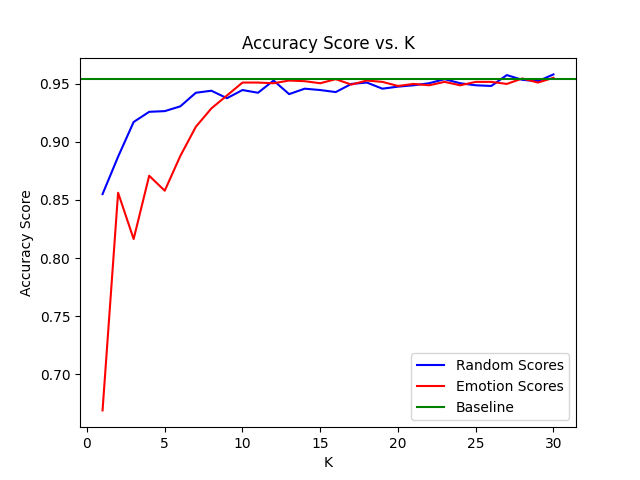
\includegraphics[width=7cm]{imgs/accuracy.png}
    \caption{Accuracy Scores as a Function of $k$}
    \label{fig:acc-scores}
\end{figure}

\begin{figure}[H]
    \centering
    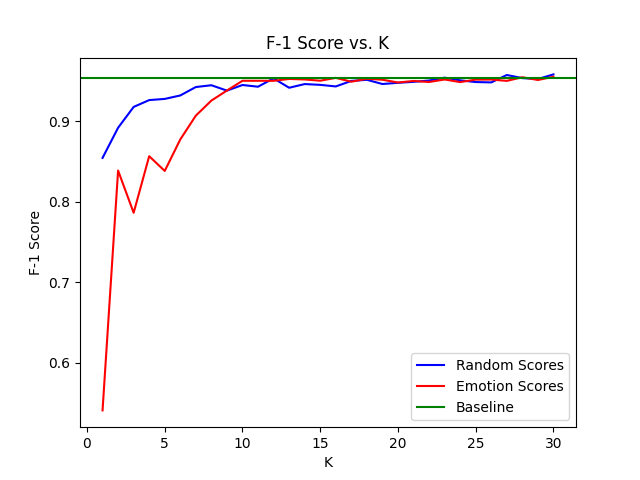
\includegraphics[width=7cm]{imgs/fscore.png}
    \caption{F-1 Scores as a Function of $k$}
    \label{fig:f1-scores}
\end{figure}

Note that the average training sample in the experimental dataset consists of about 19.15 tokens. I will compute all storage improvements generated by my models in terms the number of tokens they remove from an average sample; in other words, from the 19.15 tokens used on average. With this frame in mind, the above figures illustrate two central findings.

Firstly, Select-K-Random significantly outperforms Select-K-Weighted at low ($< 9$) values of $k$. It also still provides a reasonable basis for an effective model and produces accuracy and F-1 scores greater than 0.85, even for $k$ values as low as 2. In domains where an accuracy of 0.85 is acceptable, the Select-K-Random method would allow for a 89.5\% reduction in the size of an average training sample, which is a significant decrease in the memory commitment needed to store the model. Increasing $k$ to 5 pushes the accuracy and F-1 score above 0.9 while still reducing the memory requirements by 73.9\%.

Secondly, at $k \geq 10$, Select-K-Weighted tends to marginally outperform Select-K-Random until about $k=20$, where the performance of both models starts to converge to the benchmark. This performance boost is especially visible in the difference between the accuracies of the two models, as shown in Figure 1. Graphically, $k=10$ appears to be the optimal setting to use the Select-K-Weighted model. Increasing $k$ beyond this point adds more memory requirements while only marginally, if at all, improving the performance of the model. At $k=10$, the Select-K-Random model reduces the average size of a training sample by a factor of 0.522, which is a 47.8\% reduction in size. Therefore, if the benchmark is considered to be optimal, Select-K-Weighted produces a nearly-optimal model that uses 47.8\% less space on average.

\section{Conclusion}
This paper demonstrates the potential use of two data prepossessing methods to reduce the size of a model while maintaining similar levels of accuracy. Even a drastic reduction to two or fewer words, selected randomly, still produces a reasonable model with an F-1 and accuracy score of about 0.85. Additionally, applying the Select-K-Weighed function with $k=9$ produces a near-perfect model that reduces the size, in tokens, of the average training sample by 47.8\%. It should be noted that although the Select-K-Weighted algorithm outperforms the Select-K-Random algorithm at $k=10$, examining Figures 1 and 2 suggests that the difference is not that significant. In some domains, computing the emotional index for each word in the training dataset may be considered an unnecessary cost, at which point Select-K-Random could still be applied with $k=10$ to produce a similar, but slightly less optimal, model that achieves the same space improvements. Ultimately, these experiments suggest that the Select-K-Random and Select-K-Weighted methods are valuable tools in a context where a high-quality model is desired but memory resources may be limited.

A question left unanswered by this paper is the generalizability and optimality of the method used to compute the emotion score table. If this method is robust, it could be used to inform other sentiment analysis models, such neural network architectures that use vectorized word embeddings to perform their computations. Additionally, a better emotional score calculation technique could further improve the performance of the Select-K-Weighted model, especially at low $k$ where it performs the most poorly. Additional research into alternative techniques to calculate the emotional scores used in this paper would therefore be a highly productive contribution.
\section{Contributions}
Note that I completed this project as a team of one and was therefore responsible for all work necessary for this submission.

% Entries for the entire Anthology, followed by custom entries
\bibliography{custom}
\bibliographystyle{acl_natbib}

\end{document}
